\chapter{离子电流干扰去除}
\section{电容式离子电流检测电路的局限性}
如下图所示的是1250r/min,2000r/min,3000r/min下在30\%,40\%,50\%时的缸压和离子电流曲线。\par
\begin{figure}[H]
	\centering
	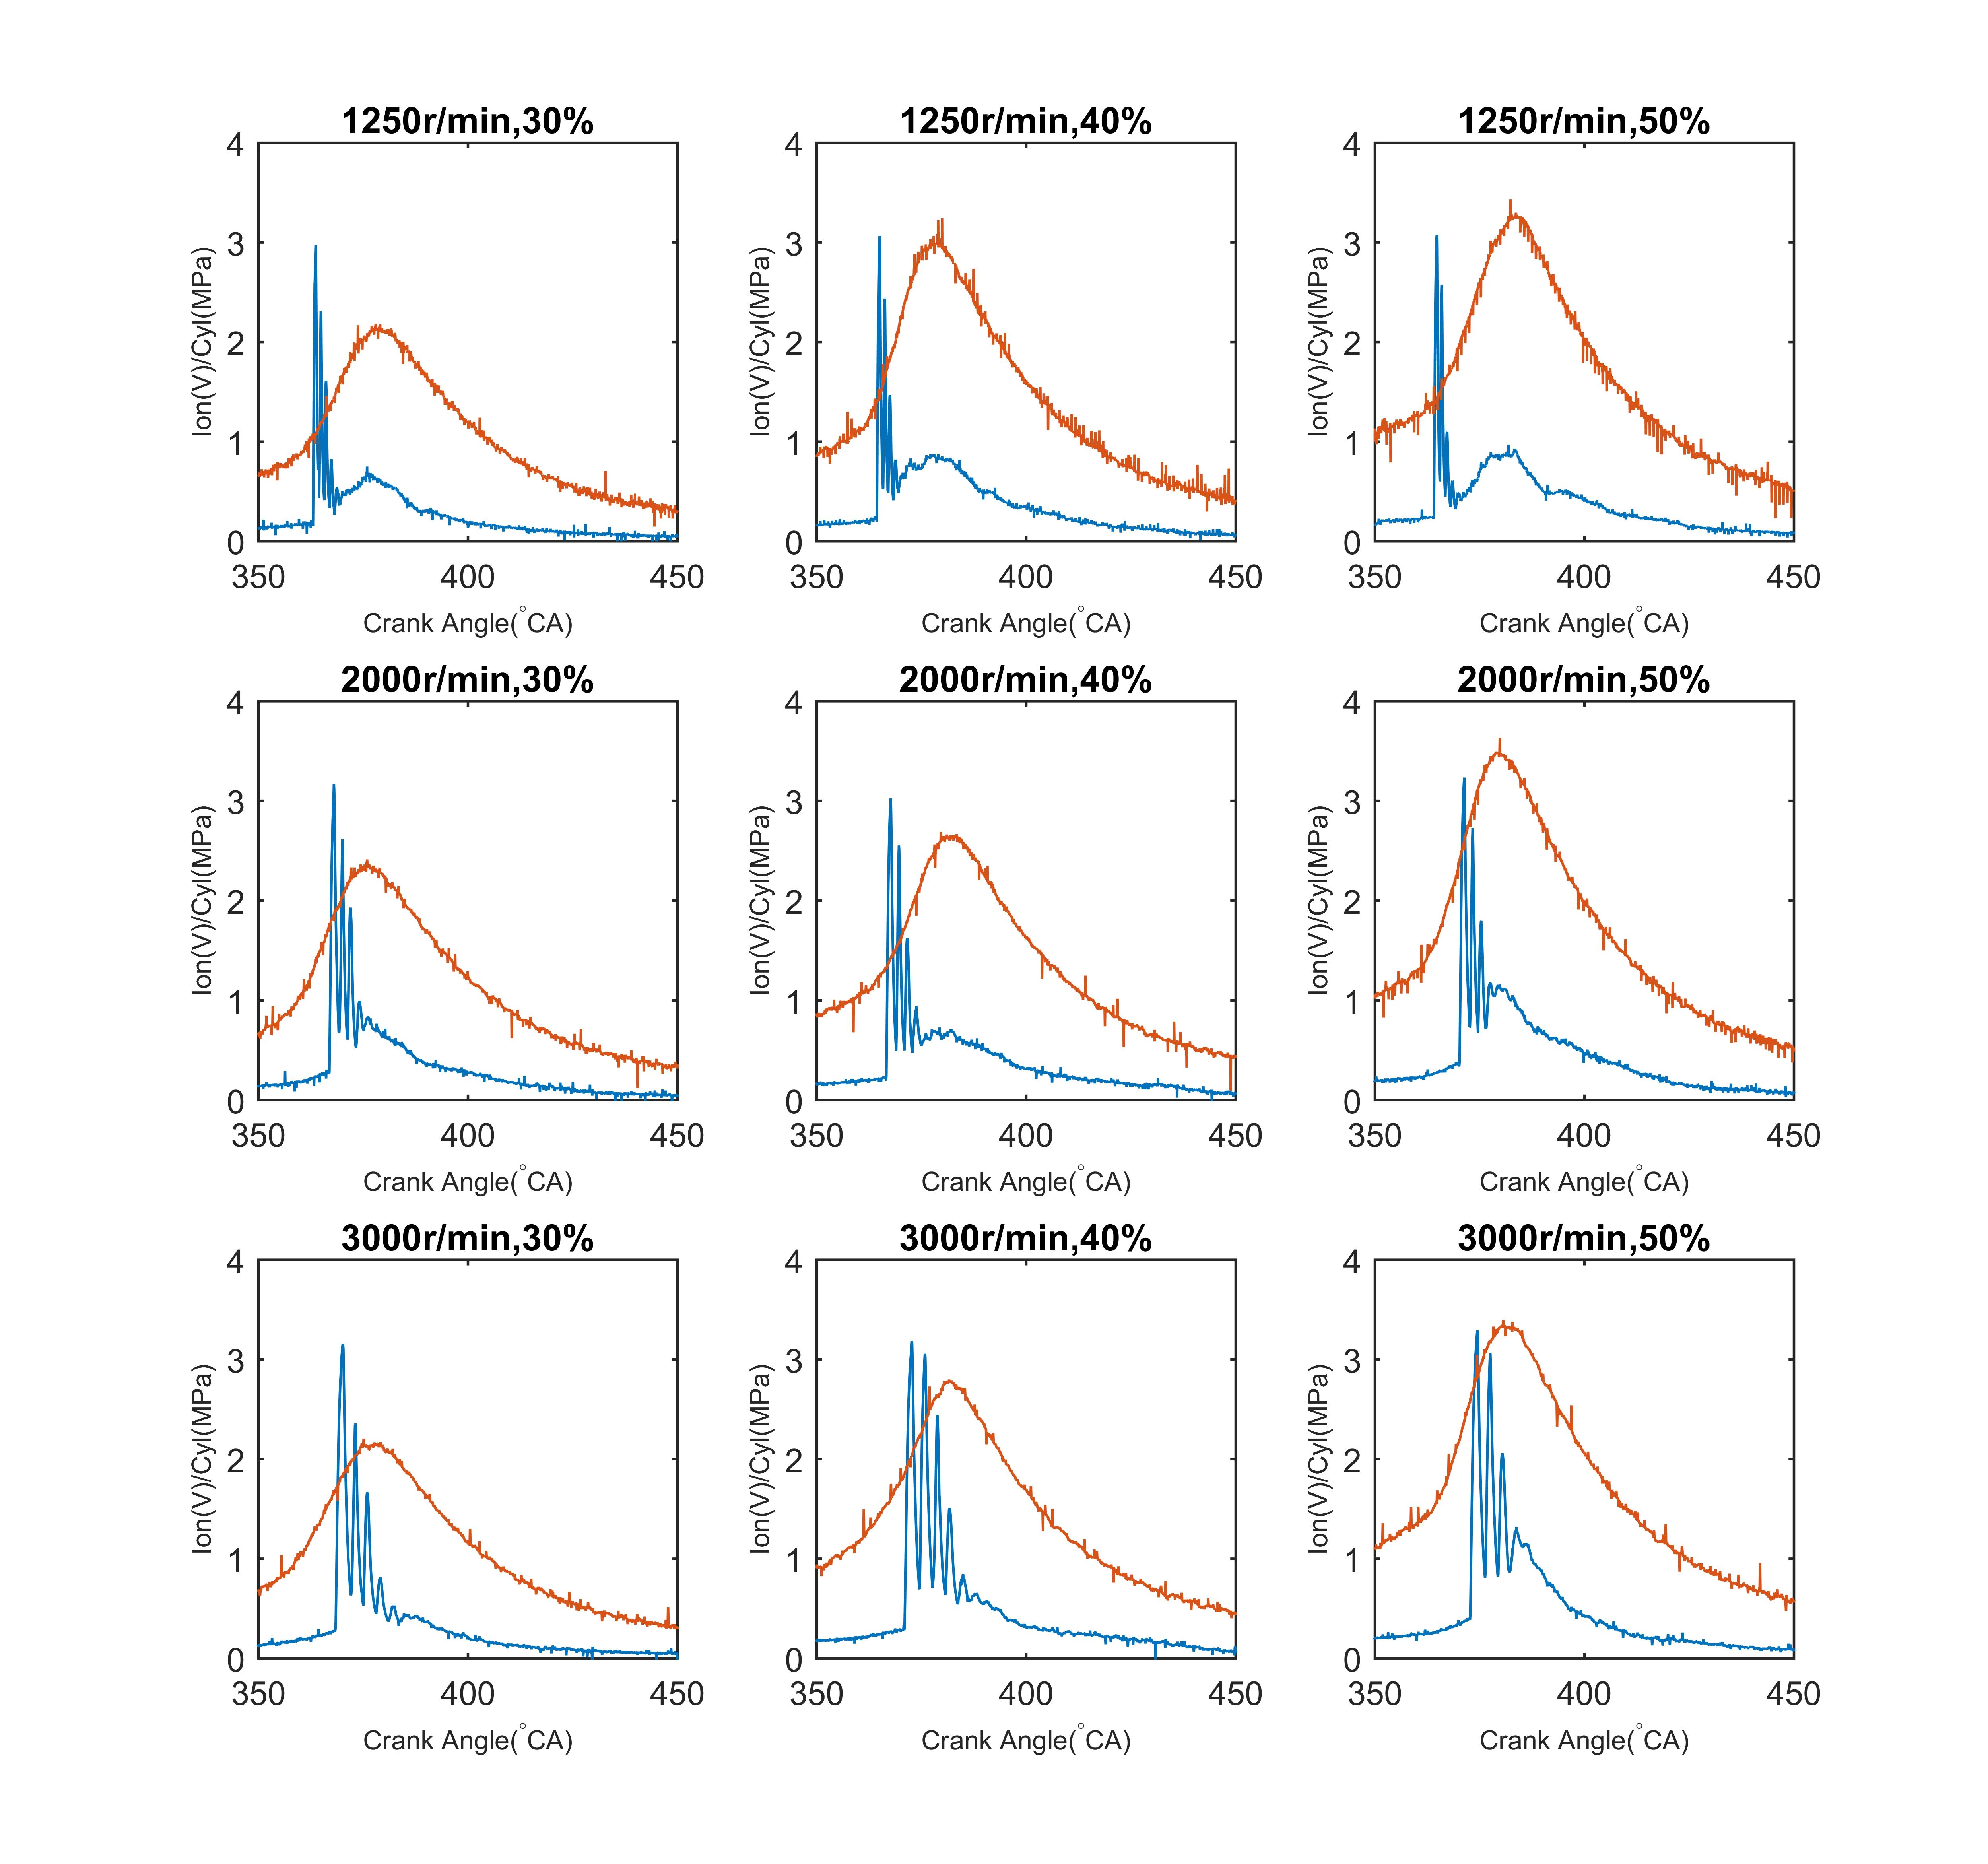
\includegraphics[width=0.9\textwidth, trim = 1cm 0.5cm 1cm 0.75cm,clip]{thesis_figure/ion_chapter/ion_vary_trending}
	\caption{不同转速、不同负荷下的缸压和离子电流}
	\label{fig:ion_cyp}
\end{figure}
从图\ref{fig:ion_cyp}中可以看到从上到下看是同一负荷下,随着转速增加的离子电流曲线;从左向右是同一转速下,随着负荷增大的离子电流曲线。
随着转速的增加,火焰后期的离子电流是逐渐被淹没的,也就是说点火干扰期将离子电流的性质淹没了,无法获得离子电流的特征值,比如离子电流的峰值及其相位就无法正常的获得。
\subsection{点火放电干扰的来源}
由于点火干扰期将离子电流的性质淹没,因此我们需要了解点火放电干扰的来源。如图\ref{fig:itf_rs}所示,左上图是200\si{\degree CA}到400\si{\degree CA}曲轴转角范围内的次级电压曲线,
左下图是200\si{\degree CA}到400\si{\degree CA}曲轴转角范围内的离子电流曲线。
通过检测次级电压来和离子电流进行对比可以发现,次级电压点火放电过程的放电干扰期和离子电流的点火干扰期重合。\par
\begin{figure}[H]
	\centering
	\includegraphics[width = 0.9\textwidth,trim=0cm 0cm 0cm 0.5cm,clip]{thesis_figure/ion_chapter/interfere_comparison}
	\caption{\label{fig:itf_rs}次级电压和离子电流对比}
\end{figure}
我们将次级电压曲线和离子电流曲线同时放大至300\si{\degree CA}到350\si{\degree CA}曲轴转角范围内的,
得到右边的两图,可以看到两者的波峰和波谷相互对应,说明两者的震荡频率是一致的。\par
由以上两张图的分析结果可以知道,离子电流的点火干扰期是由次级线圈的点火放电信号导致的,会产生一个特定频率的震荡信号。
\subsection{点火放电干扰的性质}
在单一循环中对比次级电压和离子电流可以发现点火干扰信号的来源,比较不同工况下的点火干扰信号可以分析其性质。
将不同转速下的离子电流曲线放在一起比较,可以看到如图\ref{fig:4_3_dif_rpm_ion}所示的图形。\par
\begin{figure}[htb]
	\centering
	\includegraphics[width=0.85\textwidth, trim = 1cm 0.5cm 1cm 0.5cm,clip]{thesis_figure/ion_chapter/4_3_dif_rpm_ion}
	\caption{不同转速下的离子电流按曲轴转角对比和按时间对比}
	\label{fig:4_3_dif_rpm_ion}
\end{figure}
左列的三张图从上到下为随着转速增加,离子电流按照曲轴转角进行对比,曲轴转角窗口长度为100度,可以发现点火震荡信号在不断淹没火焰前锋期和火焰后期。右列的三张图从上到下为随着转速增加,
离子电流按时间进行对比,时间窗口长度为5毫秒时间,可以发现震荡信号的频率和长度不变。
左右两列曲线分别对应了该工况下的同一个循环,由此可以知道该震荡信号具有稳定的时间长度,稳定的频率特性。
经过计算可以得到该放电周期为$0.12ms$,时长为$1ms$。\par
但是仔细观察右侧三图的波形可以看到,虽然频率和持续时间是一样的,每个波形仍然会受到干扰的影响而轻微的变形,这是干扰的不稳定特性。
\subsection{断油情况下的点火干扰分析}
\begin{figure}[htb]
	\begin{minipage}[t]{0.5\linewidth}
		\centering
		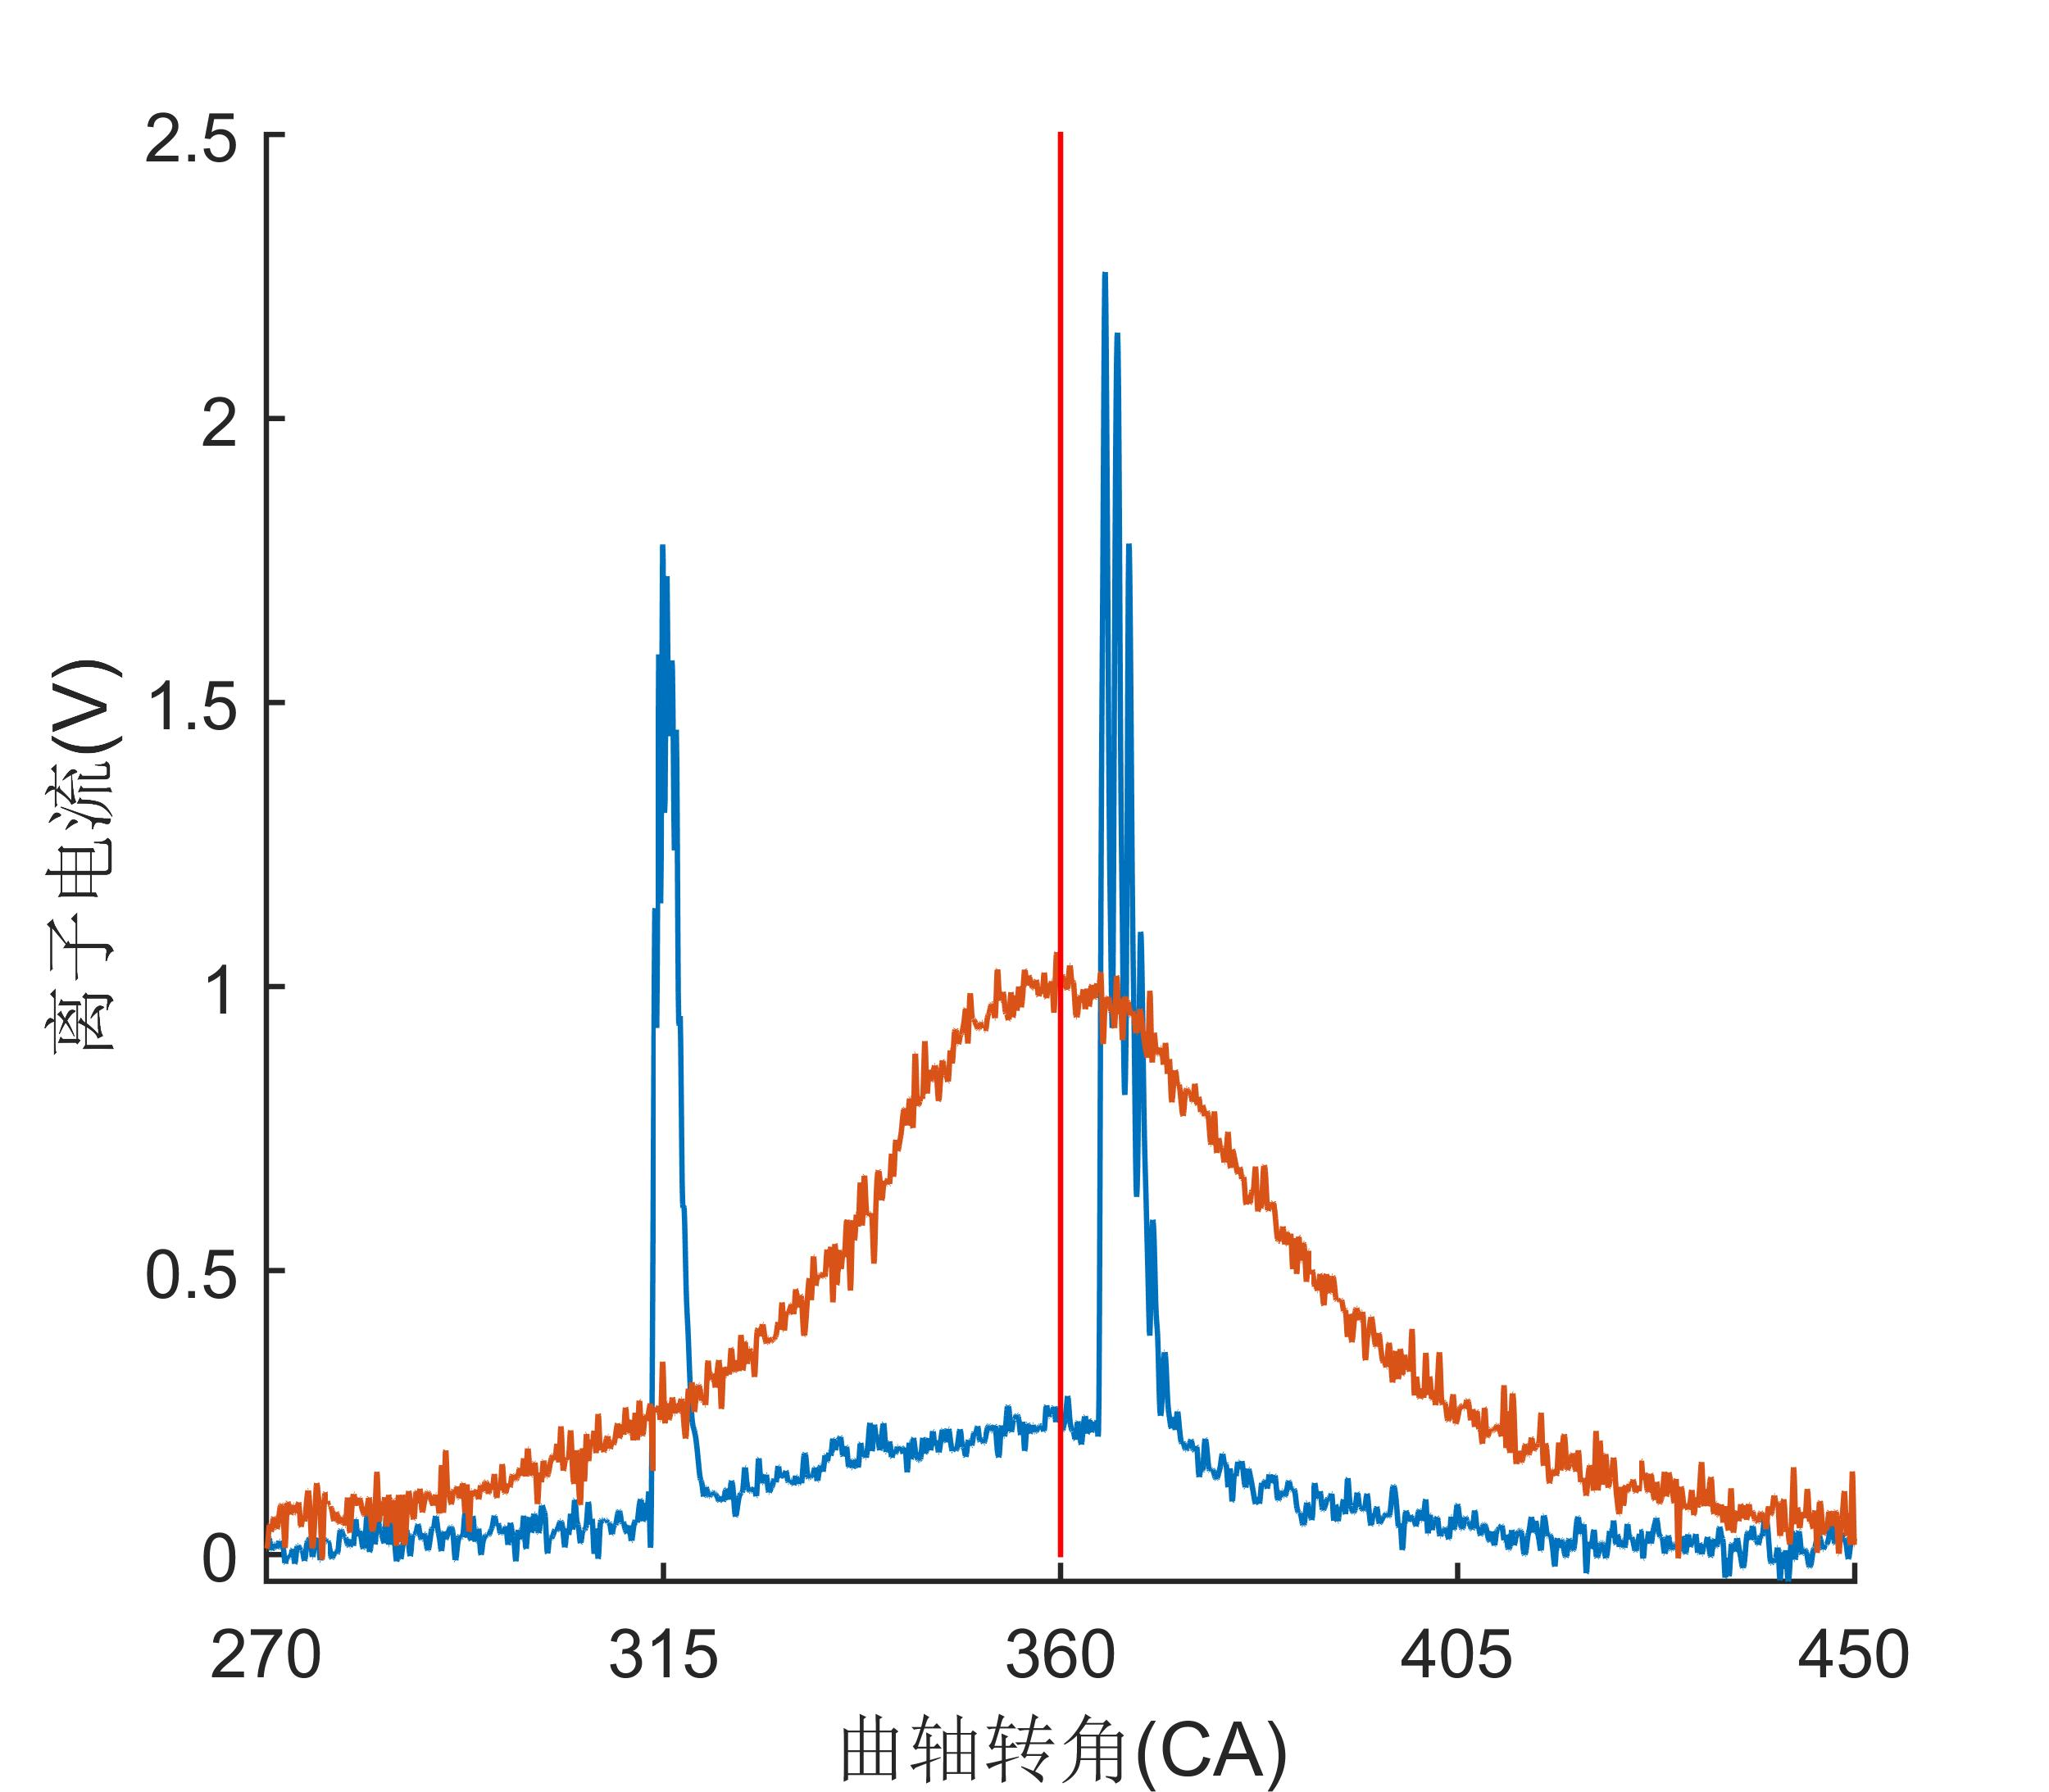
\includegraphics[width=\textwidth]{thesis_figure/ion_chapter/dy_ion}
		\caption{断油情况下的电压信号}
		\label{fig:dy_ion}
	\end{minipage}
	\begin{minipage}[t]{0.5\linewidth}
		\centering
		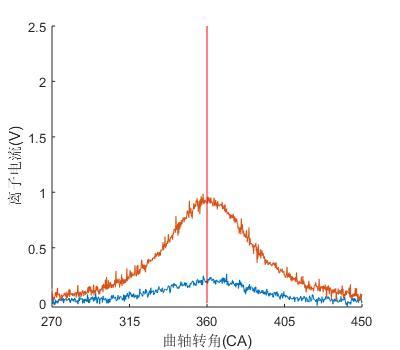
\includegraphics[width=\textwidth]{thesis_figure/ion_chapter/dh_ion}
		\caption{断火情况下的电压信号}
		\label{fig:dh_ion}
	\end{minipage}
\end{figure}
当发动机断油情况下,点火线圈仍然进行点火过程,但是缸内由于没有燃气,无法形成化学电离过程的离子电流信号,所以断油情况下的点火干扰具有稳定而且清晰的特征。\par
如图\ref{fig:dy_ion}所示是一个断油情况下的电容式检测电路检测到的电压曲线。
从图\ref{fig:dy_ion}中可以看到缸压曲线峰值相位在上止点360度位置,说明该循环处于纯压缩循环。可以看到此时的离子电流信号的峰值位置也是上止点位置,此时的离子电流信号是
热电离导致的,没有化学电离产生的离子电流信号。
\subsection{断火情况下的离子电流分析}   
当发动机断火情况下,点火线圈不进行点火过程,导致缸内混合气不能进行燃烧过程,无法形成化学电离过程的离子电流信号。如图\ref{fig:dh_ion}所示是
一个断火情况下的电容式检测电路检测到的电压信号。
从图\ref{fig:dh_ion}中可以看到缸压曲线峰值相位在上止点360度位置,说明该循环处于纯压缩循环。可以看到此时的离子电流信号的峰值相位也是上止点位置,此时的离子电流信号是热电离导致的,没有化学电离产生的离子电流信号。
\begin{figure}[htb]
	\begin{minipage}[t]{0.5\linewidth}
		\centering
		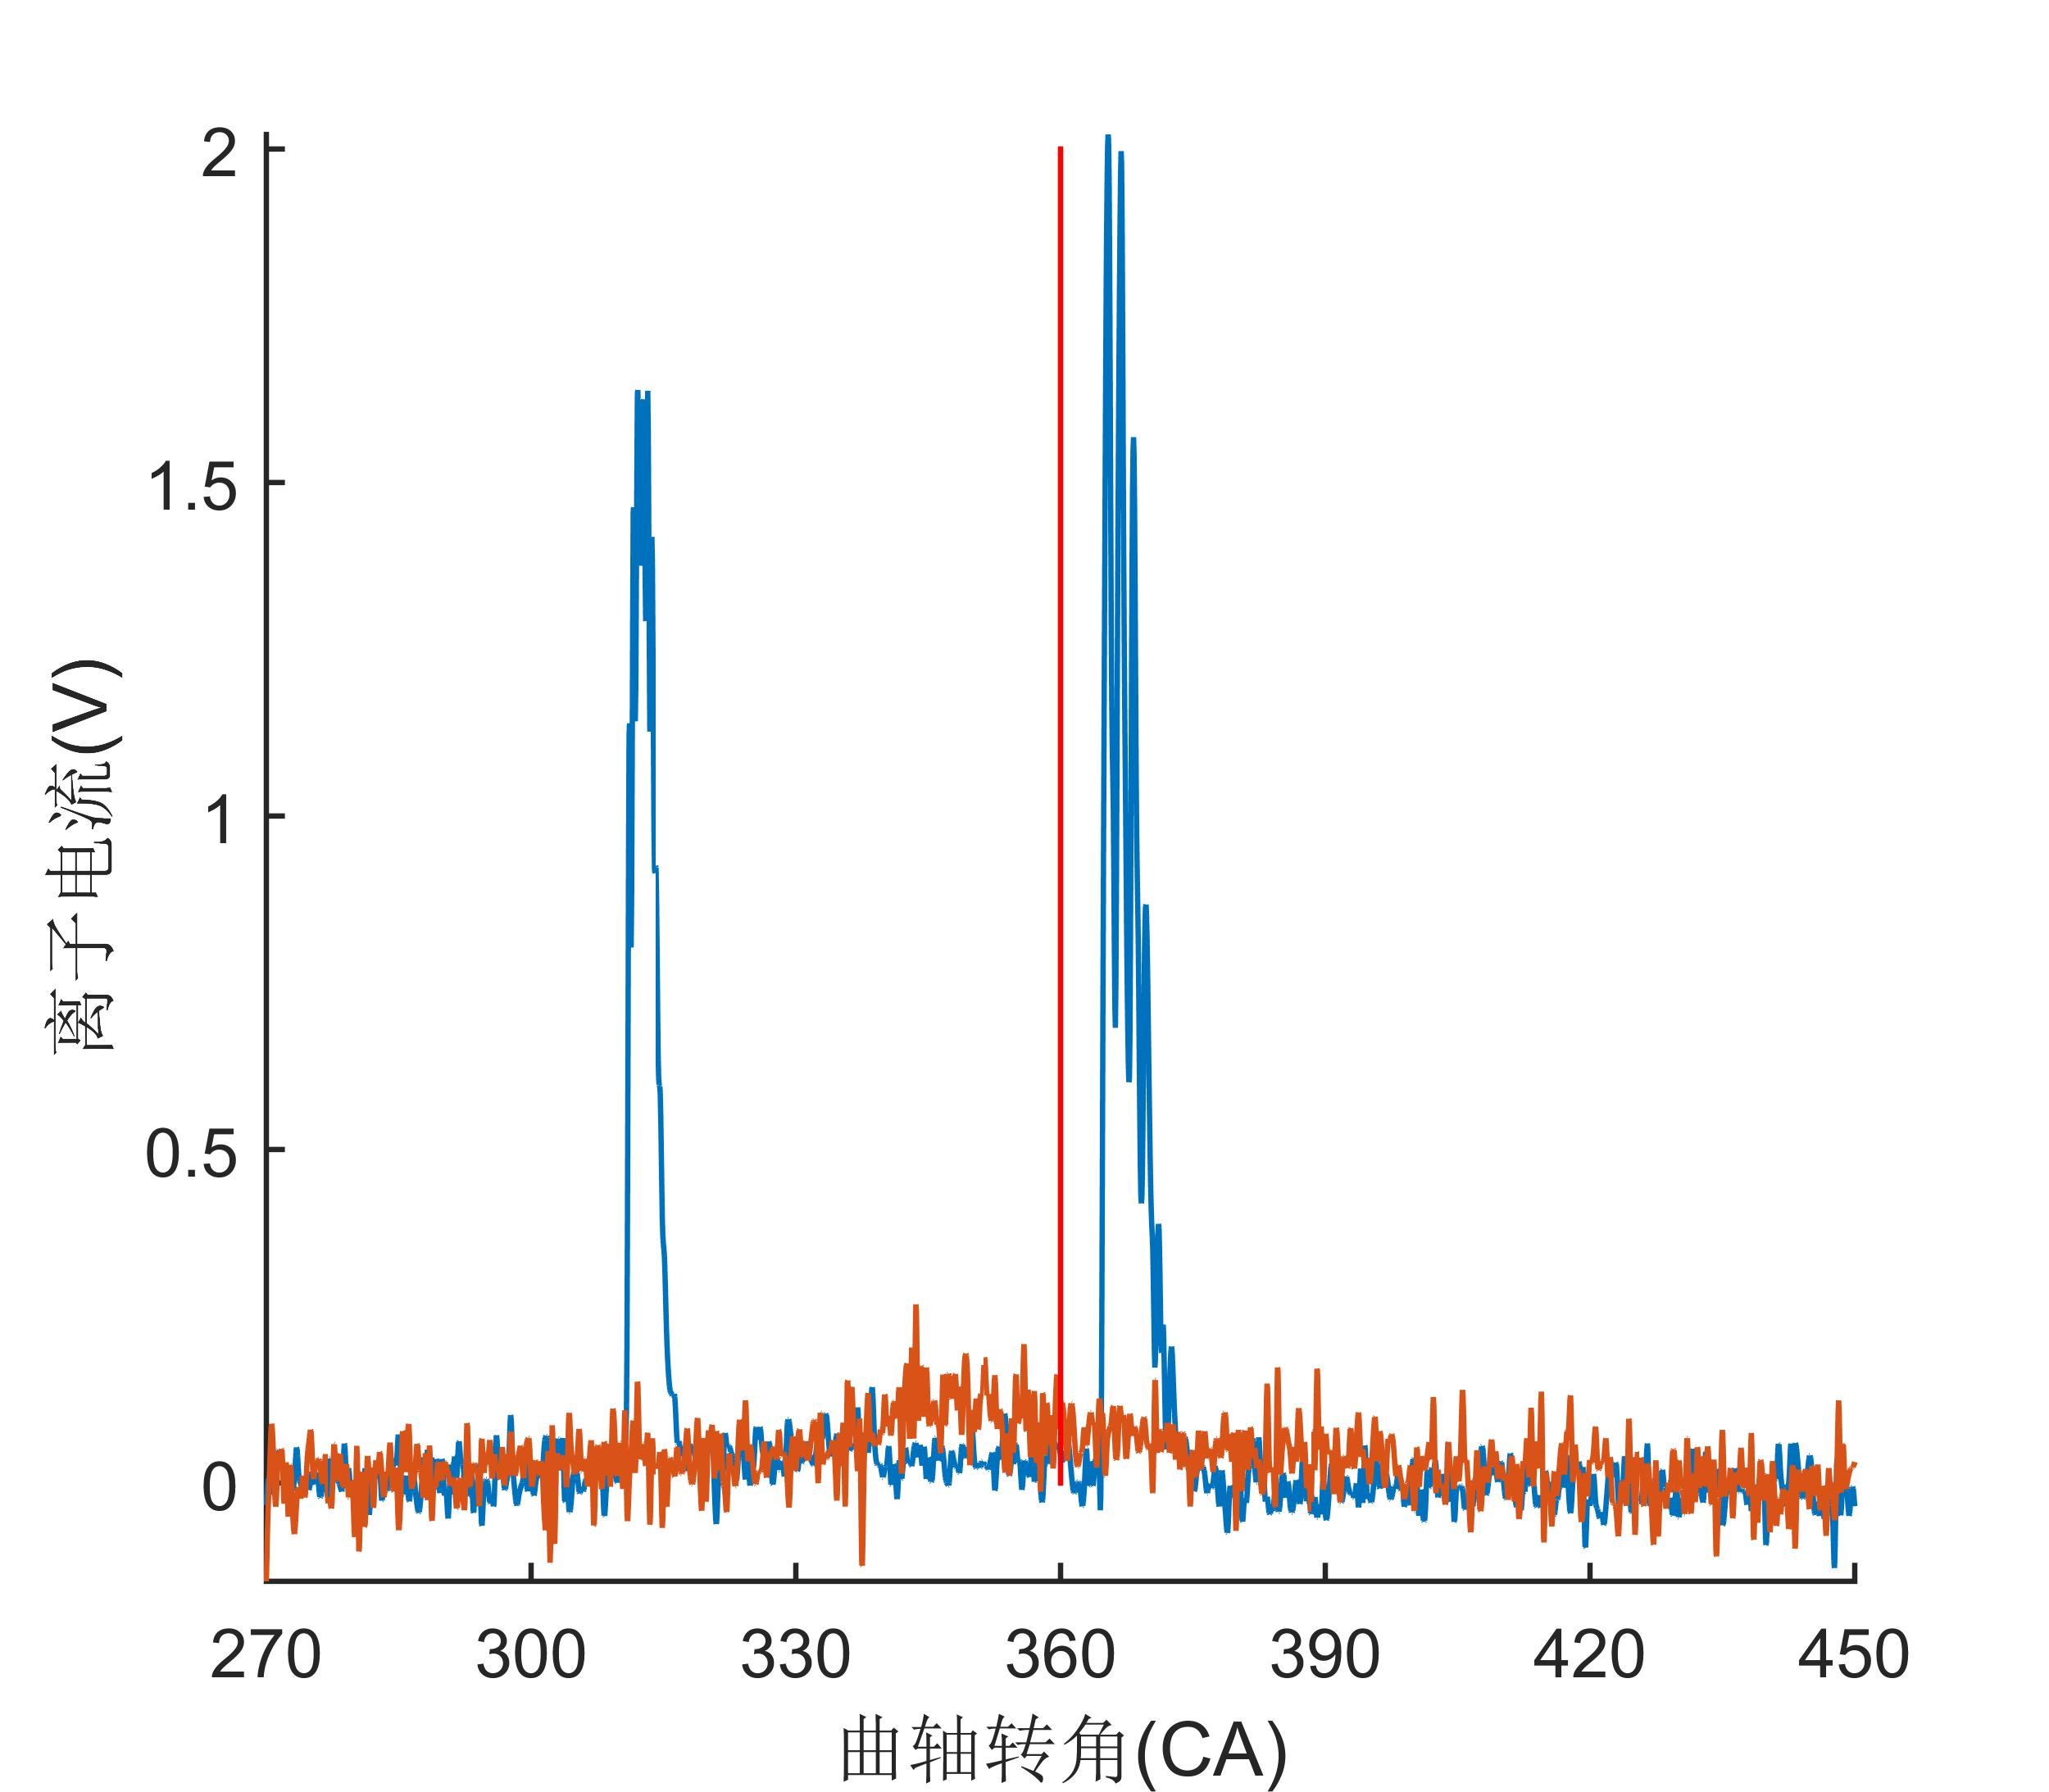
\includegraphics[width=\textwidth]{thesis_figure/ion_chapter/diff_dy_dh}
	\end{minipage}
	\begin{minipage}[t]{0.5\linewidth}
		\centering
		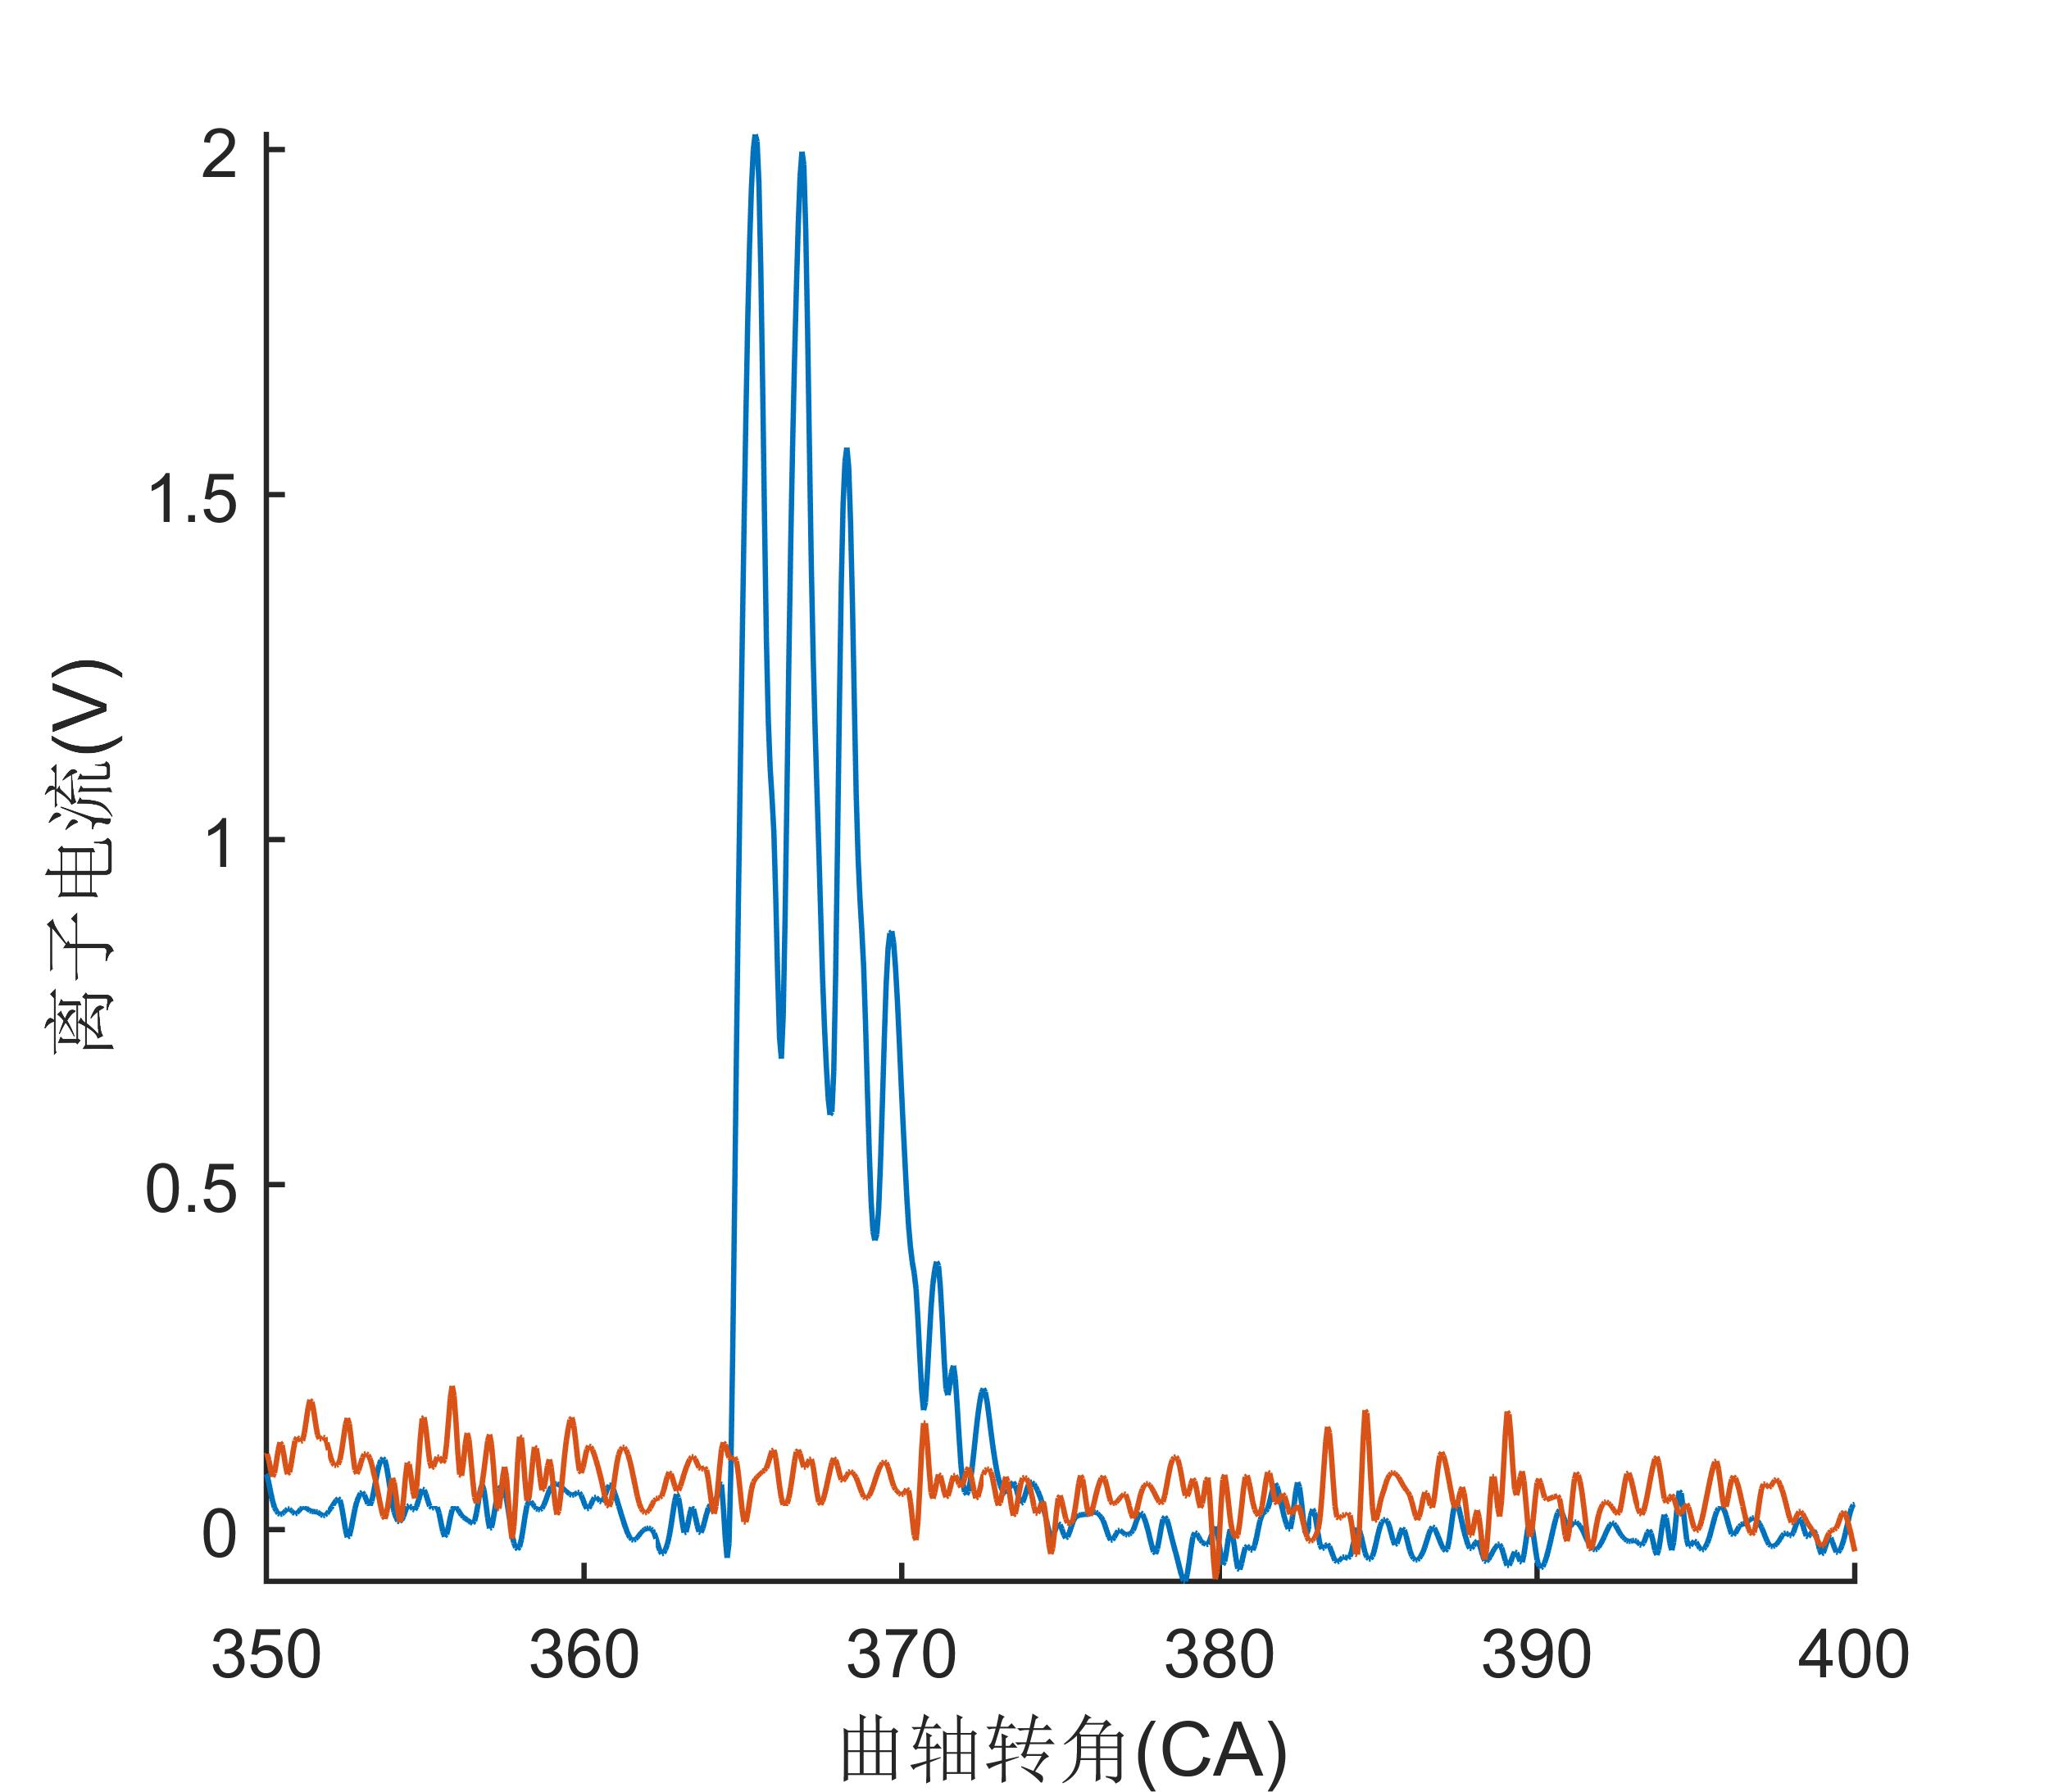
\includegraphics[width=\textwidth]{thesis_figure/ion_chapter/diff_dy_dh_detail}
	\end{minipage}
		\caption{断油离子电流信号与断火离子电流信号差值}
		\label{fig:diff_dy_dh}
\end{figure}
\subsection{纯点火干扰的分析}
对比图\ref{fig:dy_ion}和图\ref{fig:dh_ion},可以看到无论断油还是断火,都会导致缸内的混合气体无法燃烧,不能够产生化学电离,两者的循环都是纯压缩循环。
同时非NO热电离曲线的形状和峰值大小都类似。所以可以将同一转速和负荷下的离子电流信号相减,即可得到近似的纯点火干扰信号。
如图\ref{fig:diff_dy_dh}所示为差值得到的近似纯点火干扰信号,可以看到两者的缸压曲线的差值几乎为零。
\section{离子电流的小波分析方法}
\subsection{纯点火干扰信号的小波分析} 
小波分析的方法可以很好的将高频信号和低频信号进行分离,采用db,sym,coif,dmey四种离散小波基函数对纯点火干扰信号进行分析,将纯点火干扰信号中的震荡信号去除。
\begin{figure}[htb]
	\centering
	\includegraphics[width=0.9\textwidth, trim = 1cm 0.75cm 1cm 0.75cm,clip]{thesis_figure/ion_chapter/pure_ign_analysis_dmey}
	\caption{\label{fig:pure_ign_analysis_dmey}dmey小波对纯点火干扰信号小波分解}
\end{figure}
先用dmey小波对纯点火干扰信号进行10层分解,观察第二层到第七层的分解情况,可以得到如图\ref{fig:pure_ign_analysis_dmey}所示的曲线,可以看到第二层和第三层并没有将震荡信号分解开来,
而第六层和第七层分解出来的平滑信号过
于硬直,且分解的震荡信号不具有很好的衰减特性。而第四层分解相对于第五层分解来说,效果没有那么理想。\par
所以本文以下的小波分析都是基于第五层分解来进行的。由于dmey没有阶数问题,而coif小波
的最高阶数为5。因此需要确定db小波和sym小波的阶数,从而可以比较四种小波基函数对离子电流信号分析效果。
\subsection{db小波族的阶数选择和分析} 
取阶数分别为5、10、15、20、25和30的db小波对纯干扰信号进行分析。
\begin{figure}[htb]
	\centering
	\includegraphics[width=0.9\textwidth, trim = 1cm 0.75cm 1cm 0.75cm,clip]{thesis_figure/ion_chapter/pure_ign_analysis_db_order}
	\caption{\label{fig:dbvar}不同阶数下的db小波第五层分解}
\end{figure}
从图\ref{fig:dbvar}中可以看到db5和db10小波分解出来的曲线不够平滑,而从db15小波开始小波分解出来的曲线趋于一致。也就是说,
当阶数增加后,小波第五层分解的结果不变,考虑到分解阶数越多计算越加复杂。因此
db小波的阶数可以取20左右的整数值。
\subsection{sym小波族的阶数选择和分析} 
取阶数分别为5、10、15、20、25和30的sym小波对纯干扰信号进行分析。
\begin{figure}[htb]
	\centering
	\includegraphics[width=0.9\textwidth, trim = 1cm 0.75cm 1cm 0.75cm,clip]{thesis_figure/ion_chapter/pure_ign_analysis_sym_order}
	\caption{\label{fig:symvar}不同阶数下的sym小波第五层分解}
\end{figure}
从图\ref{fig:symvar}中可以看到sym5和sym10小波分解出来的震荡信号不规则,这不符合点火线圈震荡信号稳定的特征。而从sym15小波开始分解出来的曲线趋于一致。
也就是说当阶数增加到20以后,小波分析第五层分解的结果已经基本不变了,而且随着阶数的增加,sym小波分解的时间增加很快。因此
sym小波的阶数可以取20左右的整数值。\par
\subsection{小波去除纯点火干扰}
根据前面所述可以知道,采用db15,sym15,coif5和dmey小波基函数对纯点火干扰信号进行第5层分解都可以很好的将震荡信号分离出来。
小波分解方法也可以用于采集到的离子电流信号,从中可以分解出震荡和真实信号。
\begin{figure}[htb]
	\centering
	\includegraphics[width=0.9\textwidth, trim = 1cm 0.75cm 1cm 0.75cm,clip]{thesis_figure/ion_chapter/dmey_demo}
	\caption{\label{fig:dmey_realIon}dmey小波分解的真实离子电流信号}
\end{figure}
因此,去除纯点火干扰的方法为用同一个小波基函数对离子电流信号和纯点火干扰信号进行分析,可以将两者的震荡信号分别提取出来得到剩余的曲线,然后两者做差值得出理想的离子电流信号。\par
如图\ref{fig:dmey_realIon}所示的用dmey小波基函数
进行五层小波分析得到的干扰第一峰对比、干扰第二峰对比、提取震荡对比、提取真实离子电流对比以及原信号和提取信号比较图。\par
此时的工况为$1000r/min$、40\%负荷,如左侧第三图所示在此工况下热电离产生的波峰不会被点火干扰淹没。从右侧第三图中可以看到提取信号可以很好的和原离子电流的其他信号部分进行衔接。
左侧第一图显示的是干扰第一峰的对比图,可以看到纯点火干扰信号和离子电流信号的干扰第一峰相近,两者的差值几乎为零。右侧第一图显示的是干扰第二峰的对比图,可以看到两者的差值仍然存在
很强的震荡信号,和真实信号有偏差。\par
左侧第二图显示的是提取震荡的对比,可以看到从纯点火干扰中提取到的震荡信号和离子电流信号中提取到的震荡信号在频率和振幅上几乎一样,两者的差值几乎为零。
这说明了用小波分析的方法对点火干扰进行去除有很好的效果,可以提取出真实的离子电流信号出来。
\subsection{四种小波对去除点火干扰分析的比较}
如图\ref{fig:diff_wv_comp}所示是四种小波对真实离子电流进行处理后的信号比较。
从图\ref{fig:diff_wv_comp}中可以看到四种小波基函数都能够很好的将离子电流的震荡信号分离提取出平滑的曲线。\par
\begin{figure}[htb]
		\centering
		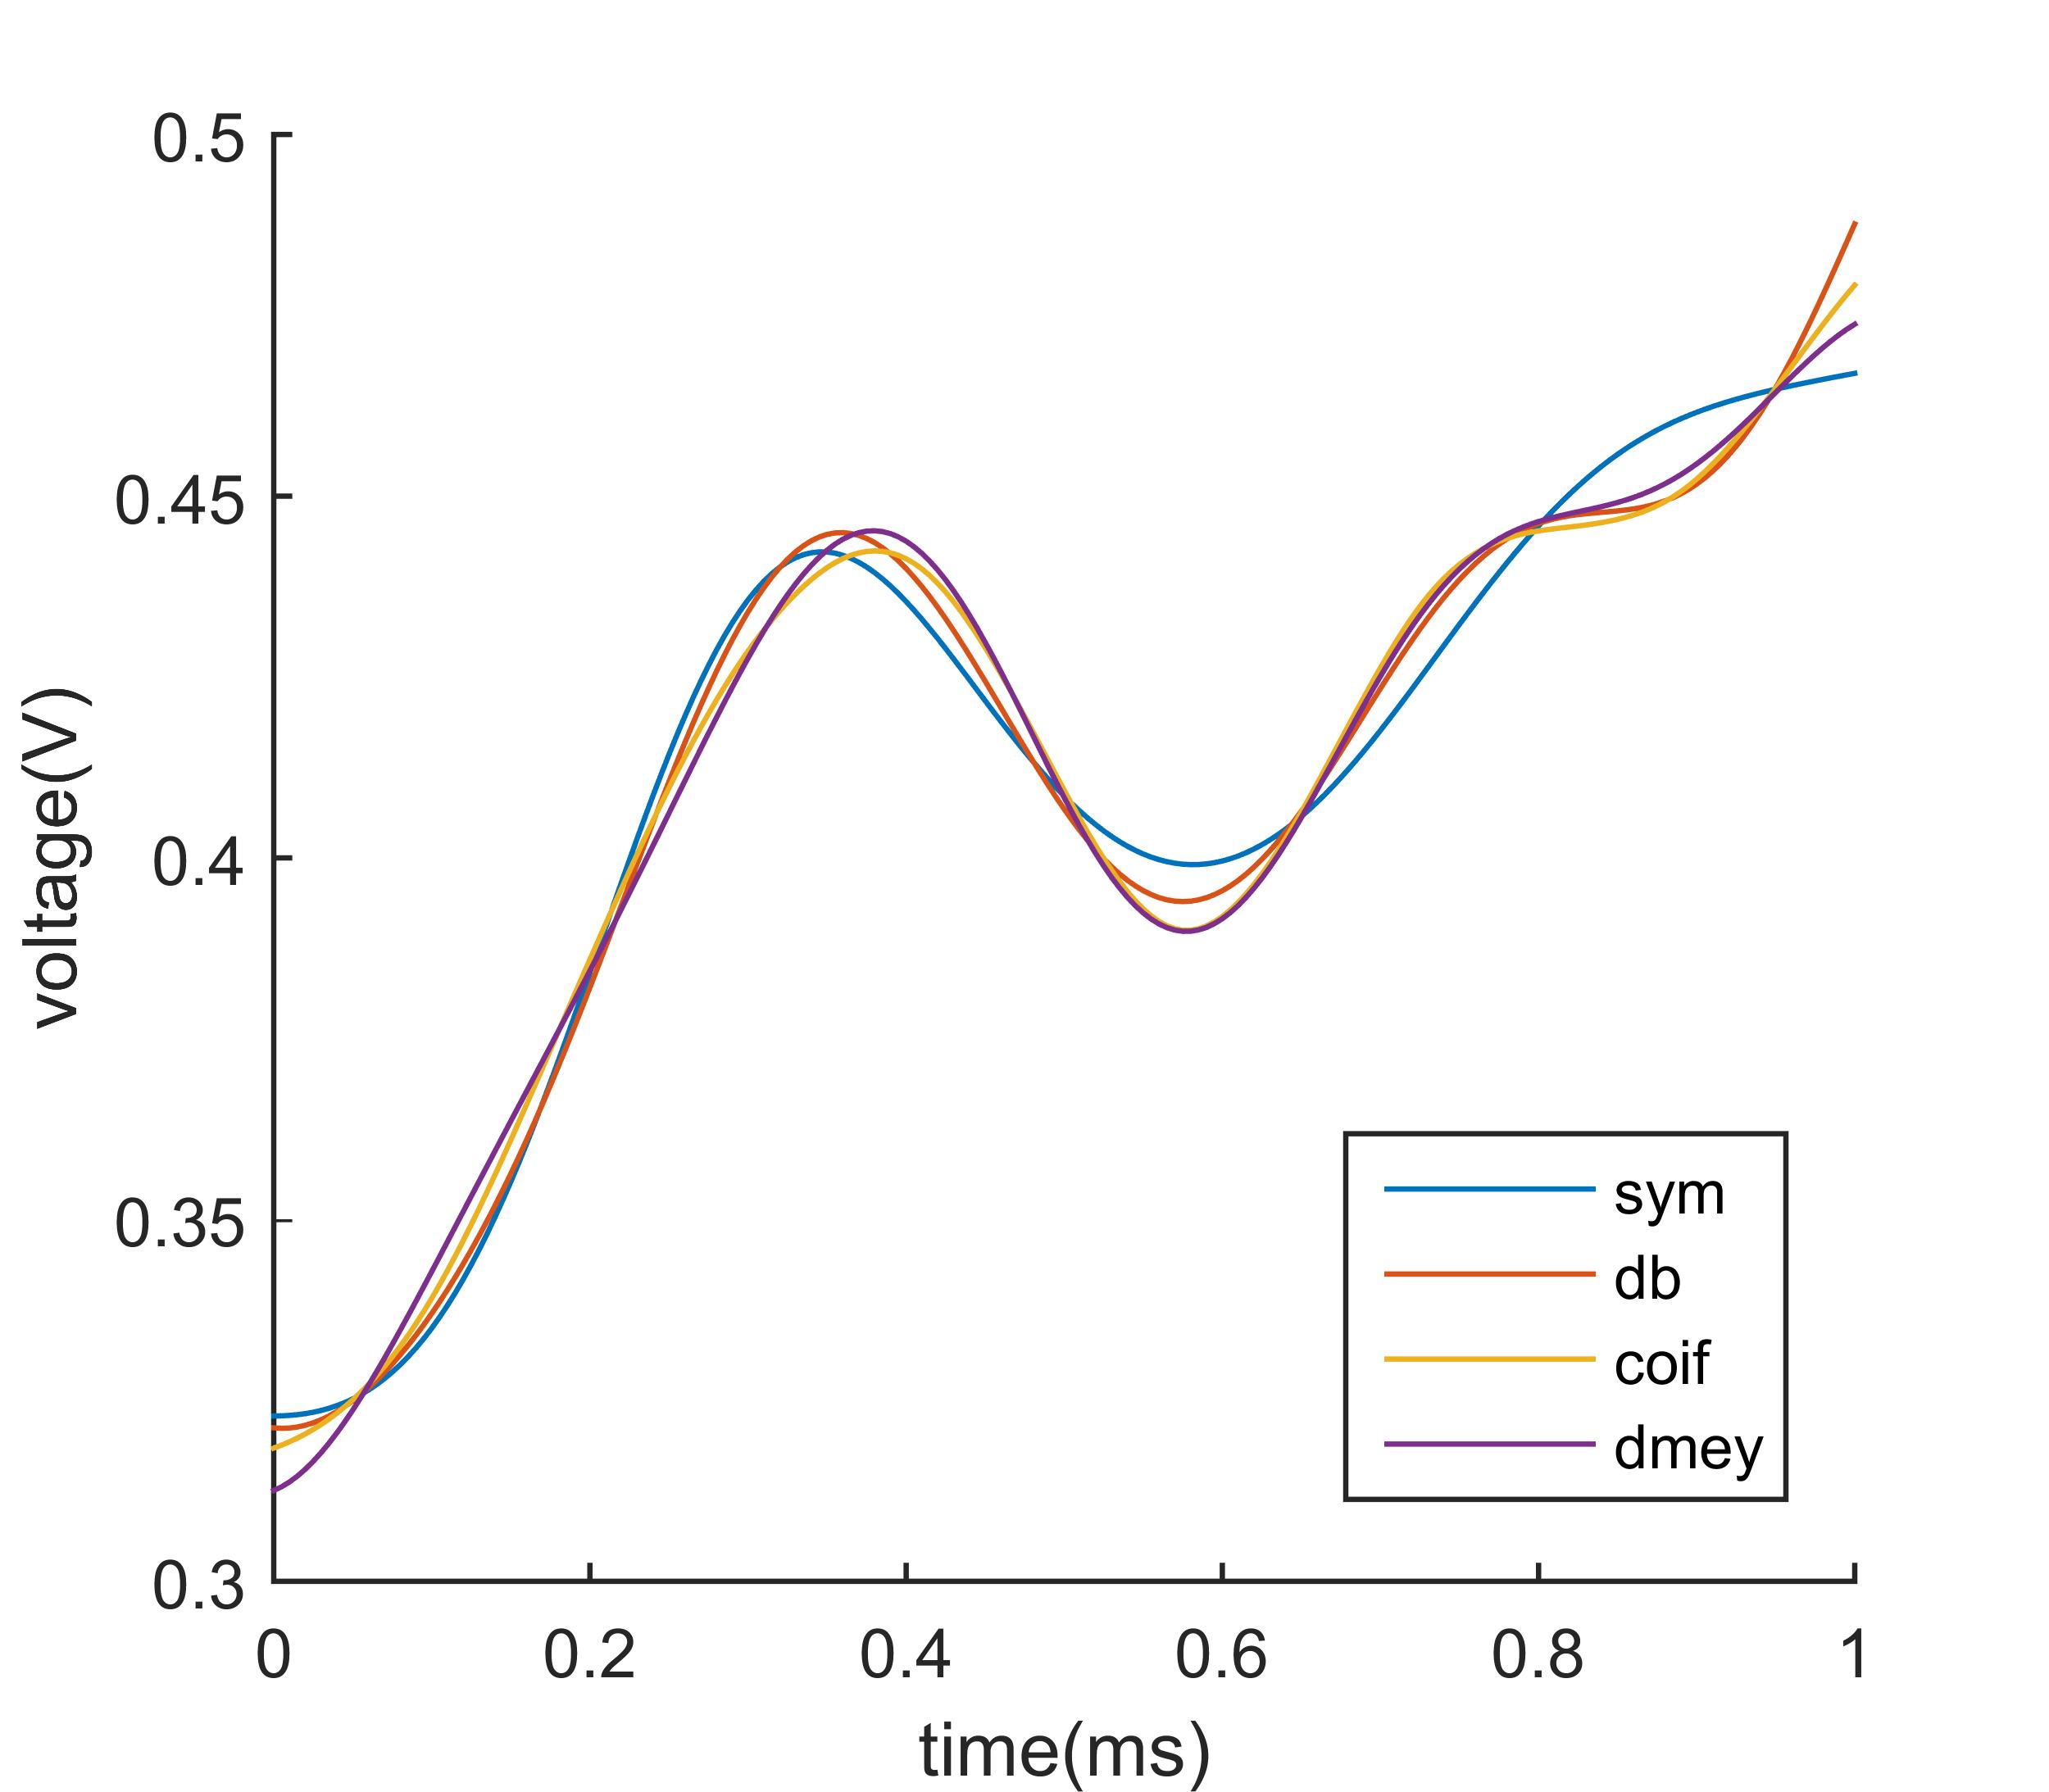
\includegraphics[width=0.75\textwidth]{thesis_figure/ion_chapter/diff_wv_comp}
		\caption{\label{fig:diff_wv_comp}四种小波对真实离子电流进行去干扰处理}
\end{figure}
但是如表\ref{wv_diff}所示的运行时间来看,从时间对比可以看出采用dmey小波函数进行小波分析的速度最快。因此在本文之后的小波基函数的选择上都采用dmey小波基
函数的第五层近似分解作为小波分析的提取结果。
\begin{table}[htb]
	\centering
	\caption{\label{wv_diff}四种小波基函数计算时间}
	\begin{tabular}{|c|c|c|}
		\hline
		小波名称&时间(s)\\\hline
		dmey & 0.002    	\\\hline
		coif & 0.008     	\\\hline
		db   & 0.019		\\\hline
		sym  & 0.131		\\\hline
	\end{tabular}
\end{table}
\section{高斯曲线拟合}
\subsection{离子电流拟合可行性}
根据第2章中的火焰后期离子电流公式推导\ref{eqn:ion_eqn},火焰后期的离子电流近似于高斯函数,可以用高斯曲线进行拟合。同时根据图\ref{fig:dy_ion}和图\ref{fig:dh_ion}可知即使在缸内无燃烧的纯压缩情况
下,仍然会有离子电流的存在,这是因为缸内存在该循环之前的循环在排气冲程未能够排除的废气。这些废气中仍然夹杂着大量的离子,且在压缩过程中随着温度升高,离子的活动变得
更加的剧烈,这类似于火焰后期的热电离过程。\par
因此该过程也能够用高斯曲线进行拟合,同时该曲线的中心位置必定在上止点曲轴转角附近。
除此之外,由于废气产生的热电离具有很明确的中心位置,因此在特定工况下,可以直接确定该废气热电离离子电流曲线对应的高斯拟合曲线,从而加快算法的计算提高拟合的速度。
\subsection{拟合算法}
双高斯曲线拟合算法的基本原理是设定两个高度为单位高度的高斯曲线的初始中心位置和宽度,通过不断计算合成的双高斯曲线和真实曲线之间的差值来确定最小差值所在位置,从而得到此时的中心
位置和宽度,所以初始值的设定非常的重要。
由于燃烧的相位通常来说在360度到420度曲轴转角左右,因此可以设一个高斯曲线的初始中心位置为380度,初始的宽度为40度;另一个
高斯曲线和缸内的废气的热电离过程有关,因此可以设置为初始中心位置为360度,初始宽度为180度。
\begin{align}
	g_{c} &= 380\\
	g_{w} &= 40\\
	g_{c}^{'} &= 360\\
	g_{w}^{'} &= 180
\end{align}
初始值设定好之后,通过初始值加上一个随机增量的方式反复计算该初始值附近的值拟合形成
的双高斯曲线和真实曲线之间的差值之和,反复计算有限次后取差值之和为最小时对应的双高斯曲线为最佳的拟合曲线。\par
计算每个高斯曲线的高度的方式采用投影计算的原理,即是将离子电流信号看作是一个一维向量$\vec{I}$,每一个高斯曲线看作是同一维度下的一个基础向量$\vec{G}$,于是将离子电流信号向量$\vec{I}$
向每一个基础高斯向量$\vec{G}$作投影计算投影矩阵的行列式的绝对值即为对应高斯曲线的高度。
\begin{align}
	g_{h} &= |det(\frac{\vec{I}}{\vec{G}})|\\
	g_{h}^{'} &= |det(\frac{\vec{I}}{\vec{G^{'}}})|
\end{align}
\subsection{拟合结果}
给定在$1750r/min$、40\%负荷时的经过小波分析去除干扰的离子电流,采用双高斯曲线拟合算法进行
双高斯曲线的拟合分析得到图\ref{fig:gas_fit_asys}所示的曲线。
\begin{figure}[htb]
	\centering
	\includegraphics[width=0.8\textwidth]{thesis_figure/ion_chapter/gas_fit_asys}
	\caption{\label{fig:gas_fit_asys}双高斯曲线拟合处理}
\end{figure}
由于发动机循环中0到270度为进气和压缩冲程,450度到540度之间基本上没有任何燃烧,540度到720度是排气冲程。所以只有在270度到450度这180度之间才有缸压和离子电流信号,这和实际
测得的信号吻合。因此曲线拟合过程可以只考虑在该相位区间中的信号。
从图\ref{fig:gas_fit_asys}中可以看到,火焰后期的峰十分的明显,但是火焰前锋期并不是明显,而只能观测到一段斜率明显的曲线。
缸内废气的纯压缩过程形成的离子电流曲线也能够很好的用高斯函数进行近似拟合,该曲线的中心位置靠近上止点位置,且其形成的原理和热电离的原理是相同的。
\section{本章总结}
本章提出了电容式离子电流检测电路的局限性所在。当转速增加时,点火干扰会将正常的离子电流信号淹没,从而无法准确获得正确的离子电流特征参数。首先从次级电压曲线角度考虑,发现次级电压中的震荡
电压信号是导致离子电流信号中存在点火干扰的直接原因。通过分析断油情况下的离子电流和断火情况下的离子电流,发现两者相减可以得到纯点火干扰信号。由于纯点火干扰信号是由于点火线圈导致的,其具有
稳定的周期和频率,因此具有稳定的特征。通过对纯点火干扰信号的研究,有助于将该信号从离子电流信号中去除。\par
离散小波函数只有db、sym、coif和dmey四种,将这四种小波基函数分别应用于纯点火干扰信号和离子电流信号中,可以将各自的震荡信号提取出来得到各自的近似信号。这两个近似信号相减得到了离子电流的真实
信号,采用该方法就能够将离子电流中的干扰进行去除。同时对比了四种小波基函数在去干扰算法中的优劣,比较结果是采用dmey小波函数有最好的效果。\par
根据离子电流的理论基础可以知道火焰后期的离子电流近似于高斯函数,同时非NO离子的热电离过程也近似于高斯函数,因此可以将整个离子电流信号用两个高斯函数进行近似拟合,便于利用高斯函数的特性
进行快速计算,节省了发动机控制系统的计算资源。\par
本章主要的结论是获得一个完整的计算模型。整个模型可以分为以下几个部分:\par
1)获取单个循环完整的离子电流信号\par
2)确定两个点火干扰起始位置以及持续时间\par
3)获取在相同工况下的断油、断火离子电流信号从而得到纯点火干扰信号\par
4)通过小波分析方法去除点火干扰\par
5)采用双高斯曲线拟合算法对离子电流的特征参数进行计算\par
整个模型计算过程适用于任何工况下的离子电流信号。\par
在整个模型的设计过程中,主要的难点在于点火干扰起始位置的确定和小波基函数的选择,因为小波分析过程主要是去除掉
离子电流信号中的震荡成分,真实的离子电流是不存在震荡成分的。而点火干扰起始位置的设定直接影响了截取下来的信号是否完全包含了所有的震荡信号;不仅如此,点火干扰起始位置
设定过早容易让小波分析过程产生偏差,将无震荡信号部分的信号假定为了存在震荡成分。\par